\documentclass[12pt,a4paper]{article}
\usepackage[utf8]{inputenc}
\usepackage{geometry}
\geometry{margin=1in}
\usepackage{hyperref}
\usepackage{graphicx}
\usepackage{booktabs}
\usepackage{longtable}
\usepackage{titlesec}
\usepackage{enumitem}
\usepackage{caption}
\usepackage{float}
\usepackage{hyperref}

\captionsetup{font=scriptsize, labelfont=scriptsize}

\titleformat{\section}{\large\bfseries}{\thesection}{1em}{}
\titleformat{\subsection}{\normalsize\bfseries}{\thesubsection}{1em}{}

\title{\textbf{Vyan — A De-PIN for EV Battery Swapping}}
\author{Parth Mittal & Abhiraj Mengade}
\date{2025-08-27}

\begin{document}

\maketitle
\thispagestyle{empty}

\begin{center}
\textbf{De-PIN • KRW stablecoin • AI-powered rebalancing • IoT-secure swap stations} \\
\vspace{1cm}
\textit{Audience: Investors, partners, station operators, regulators, developers} \\
\textit{Location focus: South Korea}
\end{center}

\maketitle
\thispagestyle{empty}

\begin{abstract}
Vyan is a decentralized EV battery swapping and De-PIN (Decentralized Physical Infrastructure Network) ecosystem designed for South Korea. 
It integrates IoT-enabled swap stations, blockchain-based battery identity, and an AI-powered inventory rebalancing agent. 
By anchoring payments to a KRW-pegged stablecoin, Vyan aligns with local regulatory, user adoption needs and promotes real world utility for the government backed stable token.
The system reduces range anxiety, improves cost efficiency for both fleet and private EV users, and creates a transparent, auditable framework for battery provenance and valuation. 
This paper outlines the problem context, technical architecture, economic model, and roadmap toward large-scale deployment in Korea’s rapidly expanding EV ecosystem.
\end{abstract}

\newpage
\tableofcontents
\newpage

\section{Executive Summary}
Vyan is a decentralized battery-swapping network designed for dense urban environments in South Korea. It combines IoT-enabled swap stations, an on-chain battery registry (De-PIN), and an AI agent that monitors and rebalances inventory across the network. Payments and incentives use a KRW-pegged stablecoin to reduce FX friction and simplify local adoption. Vyan reduces range anxiety and lowers operating costs for fleet and private EV users by enabling rapid battery swaps, rewarding renewable charging behavior, and making battery value transparent and auditable on-chain.

\section{Problem Statement}

The widespread adoption of electric vehicles (EVs) in Korea continues to face friction despite government incentives and rapidly growing consumer interest. The key barriers are not only the high capital cost of batteries but also the lack of accessible charging infrastructure, which drives range anxiety among prospective buyers. 

While battery technology is improving, the bottleneck of charging remains one of the most significant inhibitors of adoption. Building out a dense charging station network is costly and time-consuming. An alternative that has emerged globally is the concept of \textbf{battery swapping}, where users can quickly exchange a depleted battery for a fully charged one at dedicated swap stations. However, this approach brings its own unique set of challenges:

\begin{itemize}[leftmargin=1.5em]
    \item \textbf{Battery provenance and valuation:} The value of a battery is highly dependent on its usage history---including age, charge/discharge cycles, and thermal stress. Without reliable audit trails, users and operators face uncertainty in pricing and valuation, leading to inefficiency and mistrust.

    \item \textbf{Centrally Controllable Pricing:} Fleet operators have central control over pricing of swaps and can dictate the pricing without the user knowing about it.
    
    \item \textbf{Inventory and rebalancing:} Swap stations require a reliable supply of fully charged batteries, but demand fluctuates across locations and times. Managing inventory and rebalancing stock between stations is logistically complex and cost-intensive.
    
    \item \textbf{Renewable attribution:} EVs are only environmentally sustainable if the electricity used for charging is itself renewable. Tracking and verifying renewable energy usage requires trusted data sources, reliable meter attestations, and careful oracle design.
    
    \item \textbf{Ecosystem coordination:} A scalable battery swapping network requires cooperation between hardware manufacturers, software providers, and operators. Existing systems are often siloed, with vendor lock-in and lack of interoperability slowing ecosystem growth.
\end{itemize}

\section{Solution Overview}

Vyan proposes a decentralized EV battery swapping ecosystem that integrates \textbf{blockchain, IoT, and AI} to address these challenges. By combining these technologies, Vyan ensures transparency, efficiency, and scalability in a way that centralized solutions cannot.  

\begin{itemize}[leftmargin=1.5em]
    \item \textbf{On-chain Battery and Station Identity (De-PIN):} Each battery and station is assigned a cryptographic identity, with metadata such as battery age, cycle count, and provenance stored immutably on-chain. This ensures transparency, prevents tampering, and enables fair valuation during swaps.
    
    \item \textbf{IoT-enabled Stations with Signed Telemetry:} Stations are equipped with IoT modules that capture and sign real-time data on charging events, temperature, and energy source attribution. This data is transmitted securely to the blockchain, building trust in the accuracy of operational information.
    
    \item \textbf{AI Inventory Agent for Demand Forecasting and Rebalancing:} An AI-powered agent continuously monitors swap events, analyzes demand patterns, and generates rebalancing strategies. By considering proximity, traffic, renewable availability, and historical demand, the AI agent optimizes fleet-wide battery allocation, reducing operational costs and downtime.
    
    \item \textbf{KRW Stablecoin for payments and rewards:} Transactions are settled using the Korean Won–backed stablecoin, ensuring price stability and widespread use for real world utility. This makes payments seamless for consumers while enabling programmable financial incentives.
    
    \item \textbf{Account Abstraction Wallets:} To lower barriers for mainstream users, Vyan employs account abstraction and custodial wallets, ensuring a Web2-native user experience. Users can interact with the system without needing deep blockchain knowledge.
\end{itemize}


\section{Technical System Sequence}

This section describes the overall workflow of the Vyan ecosystem, from the user's interaction at a swapping station to the AI-powered monitoring and rebalancing of battery inventories across the network. The flow is divided into two phases: (i) the user journey during a battery swap, and (ii) the AI monitoring and rebalancing logic that is triggered automatically after the swap is completed.

\subsection{User Journey and Battery Swap}

When a user arrives at a Vyan-enabled battery swapping station, the following sequence occurs:

\begin{enumerate}[label=\textbf{Step \arabic*:}, wide=0pt, leftmargin=*]
    \item \textbf{QR Code Scan:} The user scans the station's QR code using the frontend application. The station confirms that the QR has been scanned successfully.
    
    \item \textbf{Session Initialization:}  
    The frontend initiates a session by sending a \texttt{POST /session/start} request to the API server, including the \texttt{station\_id} and \texttt{user\_id}.  
    The server responds with a session token, enabling authenticated interaction.  
    The frontend also queries the smart contract for station details such as available slots and current battery inventory.

    \item \textbf{Battery Insertion:}  
    The user physically inserts the discharged battery into the station and confirms this action through the application.  
    The frontend calls the smart contract to calculate the expected swap fee. The smart contract returns the estimated fee.

    \item \textbf{Payment and Swap Execution:}  
    The frontend displays the payment confirmation UI (e.g., a slider or button).  
    Once the user authorizes the swap, a \texttt{swapBattery()} transaction is executed on the smart contract. The user must pay in KRW Stable Coins.
    On confirmation, the smart contract validates payment and authorizes the release of a fully charged replacement battery.

    \item \textbf{User Confirmation and Session Completion:}  
    The frontend notifies the user that the new battery is available.  
    The station interface displays a success screen for a short period before returning to the home page.  
    The API server updates its logs to mark the session as completed.
    
    \item \textbf{Credit Rewards:}  
    The smart contract credits rewards into the user's account if the user has swapped during green hours or using fully renewable sources. These rewards can then later be used for utilitarian purposes. 
\end{enumerate}

\noindent
\begin{figure}[H]
    \centering
    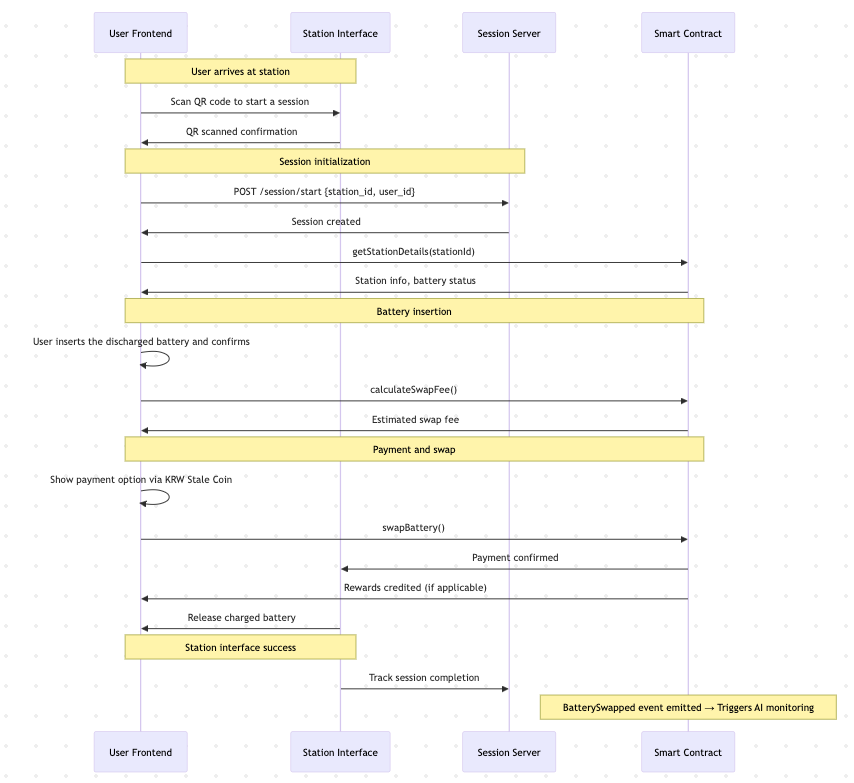
\includegraphics[width=0.9\textwidth]{diagram1.png}
    \caption{User Journey}
\end{figure}

\subsection{AI Monitoring and Rebalancing}

Following the successful swap, the smart contract emits a \texttt{BatterySwapped} event. This event acts as a trigger for the AI monitoring agent. The sequence is as follows:

\begin{enumerate}[label=\textbf{Step \arabic*:}, wide=0pt, leftmargin=*]
    \item \textbf{Event Capture:}  
    The AI agent listens for the \texttt{BatterySwapped} event from the smart contract.

    \item \textbf{Station and Network Analysis:}  
    Upon detecting the event, the AI agent queries the smart contract for the updated inventory of the affected station (\texttt{getStationDetails()}).  
    The agent also retrieves global network data (\texttt{getAllStations()}) to assess overall battery distribution.

    \item \textbf{Rebalancing Plan Generation:}  
    If a low-inventory condition is detected, the AI generates an optimal rebalancing strategy.  
    This strategy considers multiple factors such as station proximity, real-time traffic conditions, projected demand patterns, truck availability, and historical swap data.

    \item \textbf{Plan Communication:}  
    The AI agent emits an \texttt{AIRebalanceRequested} event through the smart contract.  
    The operator dashboard captures this event and displays suggested rebalancing strategies.

    \item \textbf{Station Operator Review and Execution:}  
    The operator reviews the proposed rebalancing plans and selects one.  
    Once approved, the dashboard sends the execution command to the FastAPI server.  
    The server then coordinates with station interfaces to update inventory and dispatch rebalancing operations.
\end{enumerate}

\noindent
\begin{figure}[H]
    \centering
    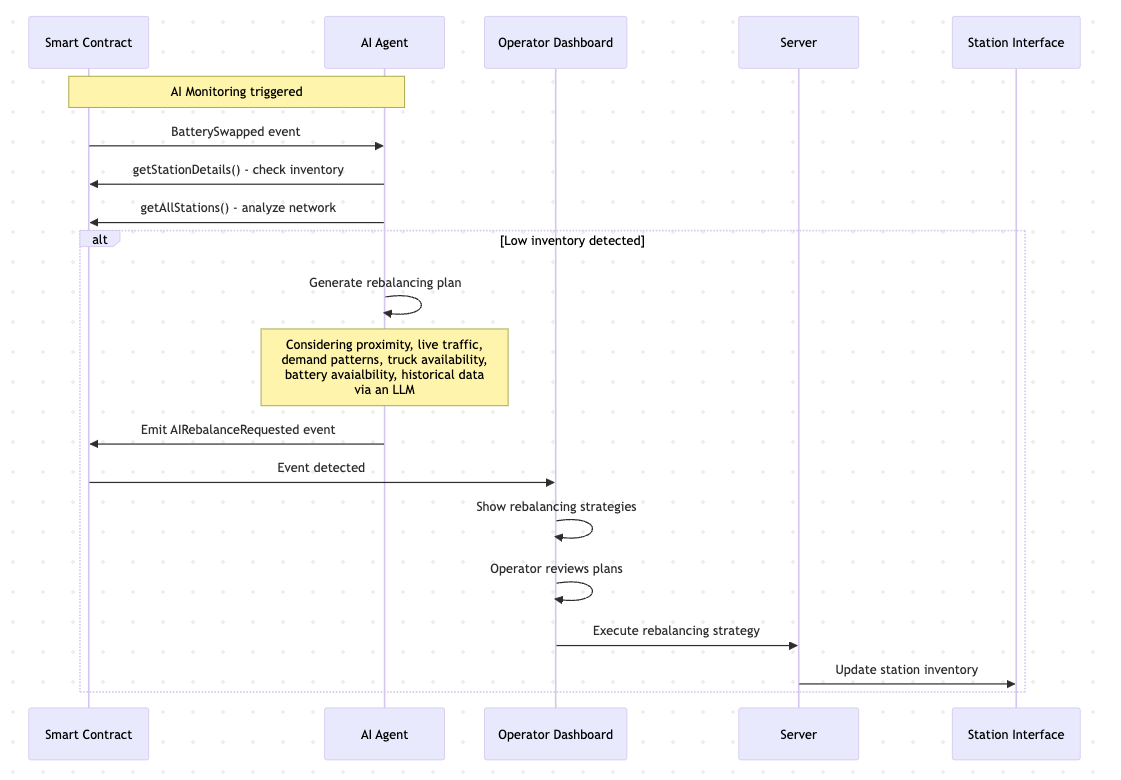
\includegraphics[width=0.9\textwidth]{diagram2.png}
    \caption{AI Powered Rebalancing for Fleet Operators}
\end{figure}


\section{Swap Price Valuation Model}
Vyan introduces a simple on-chain formula to assign fair value to each battery swap.  
The model considers a few key factors that directly affect battery health and trust:

\begin{itemize}[leftmargin=1.5em]
    \item \textbf{Age Factor ($A$):} Older batteries lose value over time. A small discount is applied each year.
    \item \textbf{Cycle Factor ($C$):} Each full charge–discharge cycle reduces value. More cycles mean lower price.
    \item \textbf{Capacity Factor ($R$):} Based on the remaining usable capacity compared to a new battery.
    \item \textbf{Energy Source Factor ($S$):} If the battery is mostly charged from renewable energy, it gets a small positive score.
\end{itemize}

We can express this in a simplified formula:

\[
V = V_{0} \times (1 - \alpha A) \times (1 - \beta C) \times R \times (1 + \gamma S)
\]

Where:
\begin{itemize}[leftmargin=1.5em]
    \item $V$ = Current value of the battery  
    \item $V_{0}$ = Base value of a new battery  
    \item $A$ = Age in years  
    \item $C$ = Number of cycles used (normalized)  
    \item $R$ = Remaining capacity fraction (0–1)  
    \item $S$ = Share of renewable energy used (0–1)  
    \item $\alpha, \beta, \gamma$ = Weight factors chosen by the protocol  
\end{itemize}

This model is lightweight, transparent, and easy to compute fully on-chain. 

\subsection{Example Calculation}

For a battery with:
\begin{itemize}[leftmargin=1.5em]
  \item Base value $V_{0} = 1{,}000{,}000$ KRW
  \item Age $A=2$ years, Cycles $C=0.20$, Capacity $R=0.82$
  \item Renewable share $S=0.80$
  \item Weights: $\alpha=0.05,\ \beta=0.30,\ \gamma=0.10$
\end{itemize}

\[
V = 1{,}000{,}000 \times (1-0.05\cdot2) \times (1-0.30\cdot0.20) \times 0.82 \times (1+0.10\cdot0.80)
\]

\[
V \approx 749{,}000\ \text{KRW}
\]

\subsection{Comparison Table}

\begin{table}[H]
\centering
\begin{tabular}{lcccc}
\toprule
\textbf{Battery} & \textbf{Age (yrs)} & \textbf{Cycles (\%)} & \textbf{Renewable (\%)} & \textbf{Value (KRW)} \\
\midrule
A (New, clean)   & 0 & 0   & 100 & 1,080,000 \\
B (Young, mixed) & 1 & 10  & 50  & 902,000   \\
C (Mid-life)     & 2 & 20  & 80  & 749,000   \\
D (Old, fossil)  & 4 & 60  & 20  & 385,000   \\
\bottomrule
\end{tabular}
\caption{Sample valuations of batteries with different ages, usage, and charging profiles.}
\end{table}


\section{Token \& Economic Model}
\subsection{Key Points}
\begin{itemize}
    \item KRWc: KRW Stablecoin for payments, rewards, operator payouts.
    \item Fee split example: Operator/Protocol/Reserve = 70/20/10
\end{itemize}


\subsection{Baseline Pilot Assumptions}
\begin{tabular}{@{}ll@{}}
\toprule
Item & Value \\
\midrule
Stations & 50 \\
Avg swaps/station/day & 8 \\
Avg swap fee (KRW) & 3,000 \\
Monthly swaps (30 days) & 12,000 \\
Monthly gross revenue (KRW) & 36,000,000 \\
\bottomrule
\end{tabular}

\subsection{Revenue Split Example}
\begin{tabular}{@{}lll@{}}
\toprule
Recipient & Share & Monthly (KRW) \\
\midrule
Operator & 70\% & 25,200,000 \\
Protocol & 20\% & 7,200,000 \\
Reserve & 10\% & 3,600,000 \\
\bottomrule
\end{tabular}

\subsection{Protocol Allocation (Example)}
\begin{tabular}{@{}lll@{}}
\toprule
Use & Share of Protocol & Monthly (KRW) \\
\midrule
Staking rewards & 50\% & 3,600,000 \\
Renewable-charge incentives & 30\% & 2,160,000 \\
Product \& ops & 20\% & 1,440,000 \\
\bottomrule
\end{tabular}

\subsection{Quick Sensitivity}
\begin{tabular}{@{}llll@{}}
\toprule
Scenario & Swaps/day & Avg fee (KRW) & Monthly revenue (KRW) \\
\midrule
Conservative & 4 & 2,000 & 12,000,000 \\
Base & 8 & 3,000 & 36,000,000 \\
Aggressive & 16 & 4,000 & 96,000,000 \\
\bottomrule
\end{tabular}


\section{Market Opportunity \& Competitive Context}

South Korea's EV market is undergoing rapid transformation, presenting a compelling opportunity for innovative solutions like Vyan.

\begin{itemize}[leftmargin=1.5em]
  \item EV penetration is accelerating — EVs are projected to account for \textbf{20\% of all vehicle sales by end of 2025}, up from just under 12\% in recent years \cite{statista-ev-sales}.
  \item Annual growth has been strong—with a compound annual growth rate (CAGR) of \textbf{19–20\% from 2020 to 2024} \cite{iea-global-ev}.
  \item The charging infrastructure is expanding rapidly: in 2025 alone, the EV charging equipment market is expected to reach \textbf{over 250 thousand installed units}, and is forecasted to grow to \textbf{over 755 thousand by 2030} (CAGR ≈ 24.7\%) \cite{mordor-charging}.
  \item On the battery front, the domestic electric vehicle battery market is also booming - estimated to reach approximately \textbf{US \$8.21 billion in 2025}, with a \textbf{CAGR greater than 16\% through 2033} \cite{mordor-battery}.
  \item Battery swapping innovations are gaining attention globally—and increasingly in Korea. For instance, Hyundai-backed pilots such as Pit In offer on-the-spot battery swaps for taxis, demonstrating real-world momentum for swap solutions \cite{hyundai-pitin}.
\end{itemize}

\section{Roadmap}
To systematically roll out Vyan’s battery swapping ecosystem, we propose the following phased roadmap:

\begin{itemize}[leftmargin=1.5em]
  \item \textbf{Q4 2025:}  
    \begin{itemize}[leftmargin=*, label=\(\bullet\)]
      \item Deploy prototype swapping station in controlled pilot region.  
      \item Launch testnet for on-chain battery and station identity tracking (De-PIN).
      \item Begin KRW-based stablecoin integration and wallet UX testing.
    \end{itemize}
  \item \textbf{Q2 2026:}  
    \begin{itemize}[leftmargin=*, label=\(\bullet\)]
      \item Initiate 10–20 station pilot across Korea in collaboration with fleet operators (e.g., taxis, deliveries).  
      \item Commence KRW stablecoin payment pilot.  
      \item Fine-tune AI rebalancing agent and IoT telemetry systems.
    \end{itemize}
  \item \textbf{Q4 2026:}  
    \begin{itemize}[leftmargin=*, label=\(\bullet\)]
      \item Scale to a commercial launch with public access to swap stations.  
      \item Begin rollout of operator dashboard and rebalancing logistics.
    \end{itemize}
  \item \textbf{2027 and Beyond:}  
    \begin{itemize}[leftmargin=*, label=\(\bullet\)]
      \item Expand network to strategic urban centers and highways.  
      \item Integrate renewable energy sources (e.g., solar + storage) at stations.  
      \item Seek partnerships with domestic battery manufacturers and logistics fleets.
    \end{itemize}
\end{itemize}


% \subsection{Suggested API Endpoints}
% \begin{itemize}
%     \item POST /session/start \{ station\_id, user\_id \}
%     \item POST /station/telemetry (signed payload)
%     \item GET /station/:id/status
% \end{itemize}



% \section{Appendices}
% \subsection{Smart Contract Interfaces}
% \begin{itemize}
%     \item registerStation(address operator, string metadataURI)
%     \item registerBattery(uint256 tokenId, bytes metadataHash)
%     \item calculateSwapFee(uint256 batteryTokenId, uint256 stationId)
%     \item event BatterySwapped(uint256 stationId, uint256 batteryTokenId, address user)
% \end{itemize}


\begin{thebibliography}{9}
\bibitem{statista-ev-sales} Statista, \emph{Electric vehicle sales share in South Korea 2015–2025}, \url{https://www.statista.com/statistics/1260143/south-korea-ev-sales-share/}

\bibitem{iea-global-ev} IEA, \emph{Global EV Outlook 2024}, \url{https://www.iea.org/reports/global-ev-outlook-2024}

\bibitem{mordor-charging} Mordor Intelligence, \emph{South Korea EV Charging Equipment Market}, \url{https://www.mordorintelligence.com/industry-reports/south-korea-ev-charging-equipment-market}

\bibitem{mordor-battery} Mordor Intelligence, \emph{South Korea EV Battery Market}, \url{https://www.mordorintelligence.com/industry-reports/south-korea-electric-vehicle-battery-market}

\bibitem{hyundai-pitin} Hyundai Motor Group, \emph{Pit In Battery Swap Pilot}, \url{https://www.hyundai.com/worldwide/en/company/newsroom}
\end{thebibliography}

\end{document}